\documentclass[12pt]{article}
\usepackage{fullpage}
\usepackage[top=10mm, bottom=45mm, left=10mm, right=10mm]{geometry}
\usepackage{amsmath,amsthm,amssymb}
\usepackage{lastpage}
\usepackage{enumerate}
\usepackage{fancyhdr}
\usepackage{xcolor}
\usepackage{graphicx}
\usepackage{listings}
\usepackage{hyperref}
\usepackage{answers}
\usepackage{setspace}
\usepackage{enumitem}
\usepackage{multicol}
\usepackage{mathrsfs}
\usepackage{algorithmic}
\usepackage{stmaryrd}
\usepackage[ruled,linesnumbered,vlined]{algorithm2e}
\usepackage{tikz}
 \usepackage{fancyvrb}
\usetikzlibrary{automata, positioning}
\usepackage{minted}
\sloppy
\definecolor{lightgray}{gray}{0.5}
\setlength{\parindent}{0pt}


\hypersetup{%
  colorlinks=true,
  linkcolor=blue,
  linkbordercolor={0 0 1}
}

\lstdefinestyle{Python}{
    language        = Python,
    frame           = lines, 
    basicstyle      = \footnotesize,
    keywordstyle    = \color{blue},
    stringstyle     = \color{green},
    commentstyle    = \color{red}\ttfamily
}

\setlength{\parindent}{0.0in}
\setlength{\parskip}{0.05in}

\newcommand\course{\textbf{EE 456}}   
\newcommand\name{Aishwarye Omer}     

\pagestyle{fancyplain}
\headheight 35pt
\lhead{\name\\\course{}}
\chead{\textbf{\Large Homework - 17}}
\rhead{\today}
\lfoot{}
\cfoot{}
\rfoot{\small\thepage}
\headsep 1.5em

\newlength\myindent
\setlength\myindent{2em}
\newcommand\bindent{%
  \begingroup
  \setlength{\itemindent}{\myindent}
  \addtolength{\algorithmicindent}{\myindent}
}
\newcommand\eindent{\endgroup}
\definecolor{codegreen}{rgb}{0,0.6,0}
\definecolor{codegray}{rgb}{0.5,0.5,0.5}
\definecolor{codepurple}{rgb}{0.58,0,0.82}
\definecolor{backcolour}{rgb}{0.95,0.95,0.92}

%Code listing style named "mystyle"
\lstdefinestyle{mystyle}{
	backgroundcolor=\color{backcolour},   commentstyle=\color{codegreen},
	keywordstyle=\color{magenta},
	numberstyle=\tiny\color{codegray},
	stringstyle=\color{codepurple},
	basicstyle=\ttfamily\footnotesize,
	breakatwhitespace=false,         
	breaklines=true,                 
	captionpos=b,                    
	keepspaces=true,                 
	numbers=left,                    
	numbersep=5pt,                  
	showspaces=false,                
	showstringspaces=false,
	showtabs=false,                  
	tabsize=2
}

%"mystyle" code listing set
\lstset{style=mystyle}

\newenvironment{solution}[1][Solution]{\begin{trivlist}
\item[\hskip \labelsep {\bfseries #1}]}{\end{trivlist}}


\begin{document}

\textbf{Question:} Use the curve fitting facility in the MATLAB NN Tool Box to approximate the graph of where $Y \ = \ sin^n(t)$ where $n$ is the 4th digit of your student ID number.

\BlankLine
\BlankLine

\textbf{Solution:} 
\BlankLine
$\bullet$ Student ID: 930616252, fourth digit = 6.\BlankLine
$\bullet$ Train the network for $Y \ = \ sin^6(t)$. \BlankLine
$\bullet$ Since it is even power, $Y \geq 0$. \BlankLine
$\bullet$ Following is the code:


 \begin{verbatim}
	% Solve an Input-Output Fitting problem with a Neural Network
	% Script generated by NFTOOL
	%
	% This script assumes these variables are defined:
	%
	%   houseInputs - input data.
	%   houseTargets - target data.
	
	inputs = -2*pi:0.01:2*pi;
	targets = sin(inputs).^6;
	
	% Create a Fitting Network
	hiddenLayerSize = 10;
	net = fitnet(hiddenLayerSize);
	
	% Set up Division of Data for Training, Validation, Testing
	net.divideParam.trainRatio = 70/100;
	net.divideParam.valRatio = 15/100;
	net.divideParam.testRatio = 15/100;
	
	% Train the Network
	[net,tr] = train(net,inputs,targets);
	
	% Test the Network
	outputs = net(inputs);
	errors = gsubtract(outputs,targets);
	performance = perform(net,targets,outputs);
	
	% View the Network
	view(net)
	
	% Plots
	% Uncomment these lines to enable various plots.
	figure, plotperform(tr)
	% figure, plottrainstate(tr)
	% figure, plotfit(targets,outputs)
	% figure, plotregression(targets,outputs)
	% figure, ploterrhist(errors)
\end{verbatim}

\begin{figure}[h]
	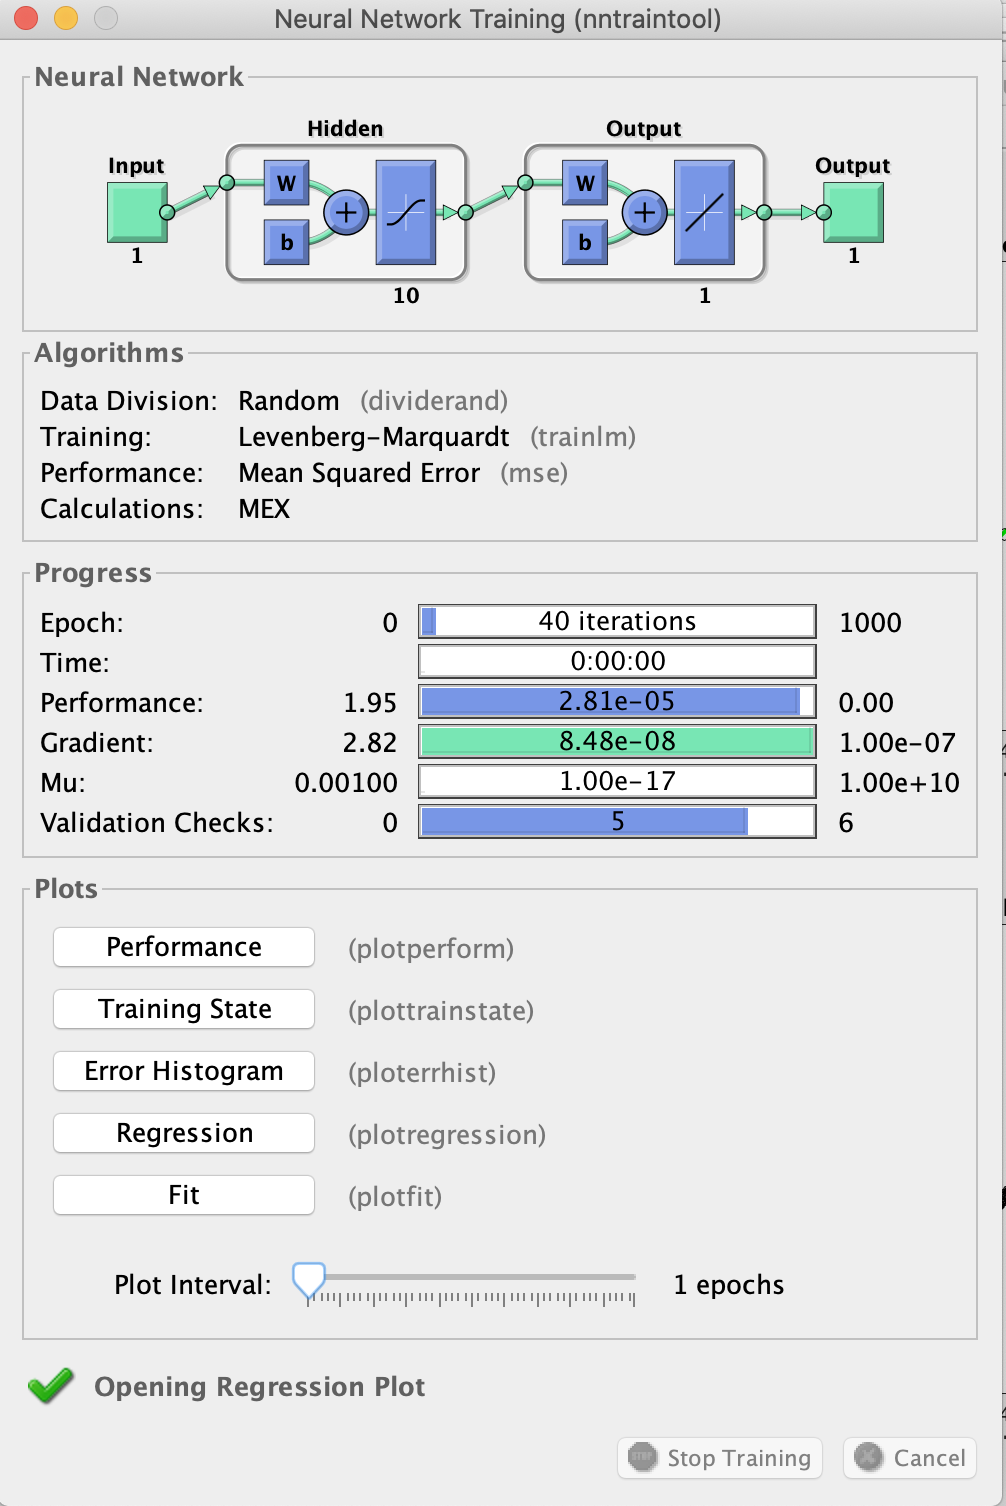
\includegraphics[width=11cm]{Main.png}
\end{figure}

\begin{figure}[h]
	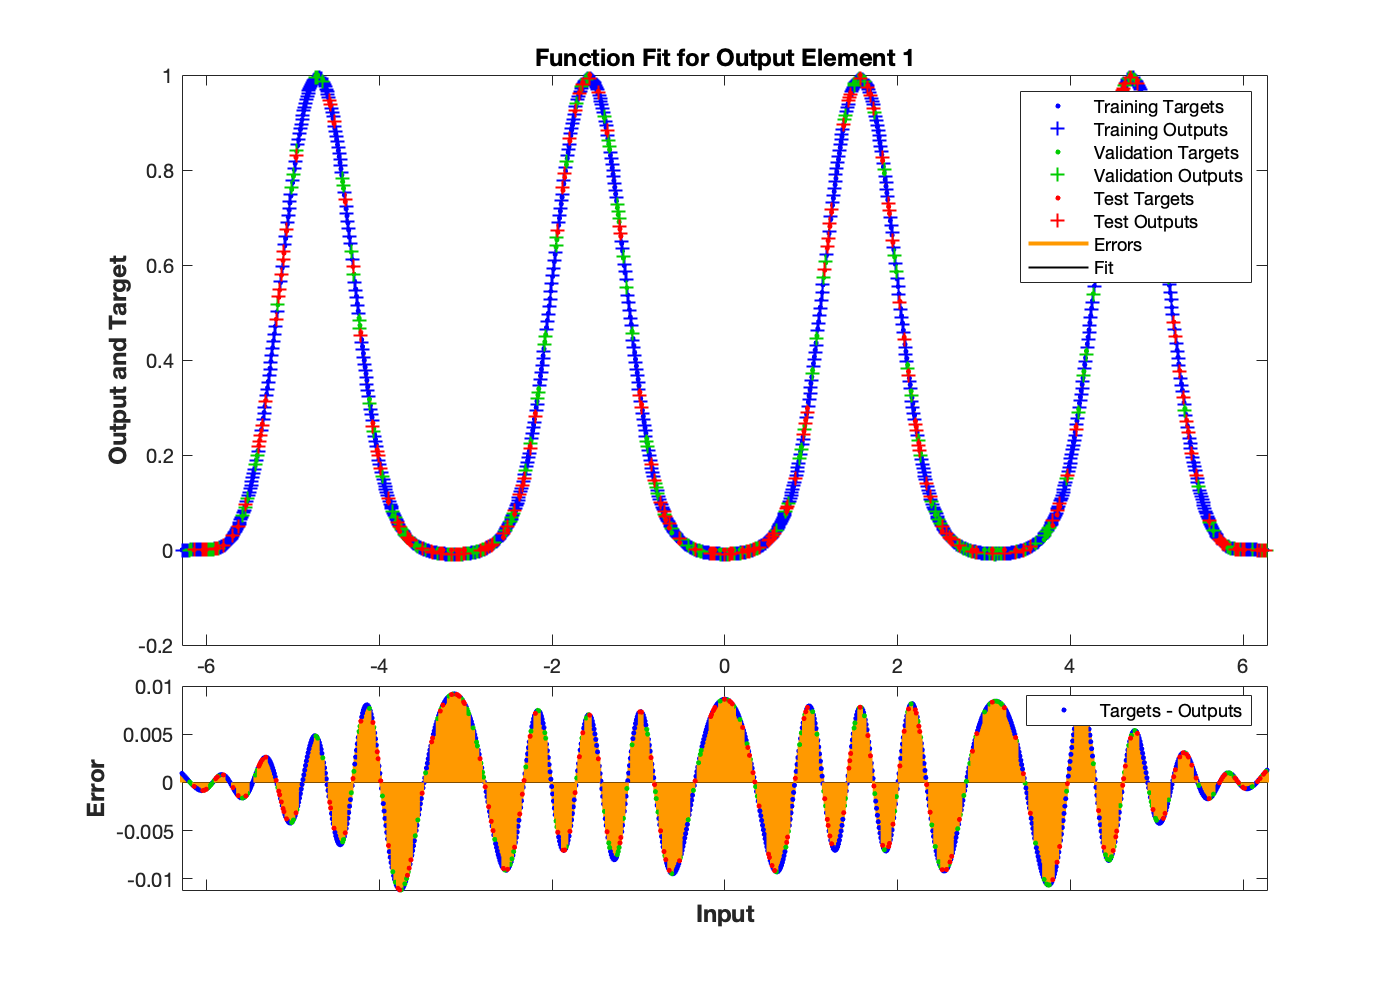
\includegraphics[width=20cm]{Graph.png}
\end{figure}

\begin{figure}[h]
	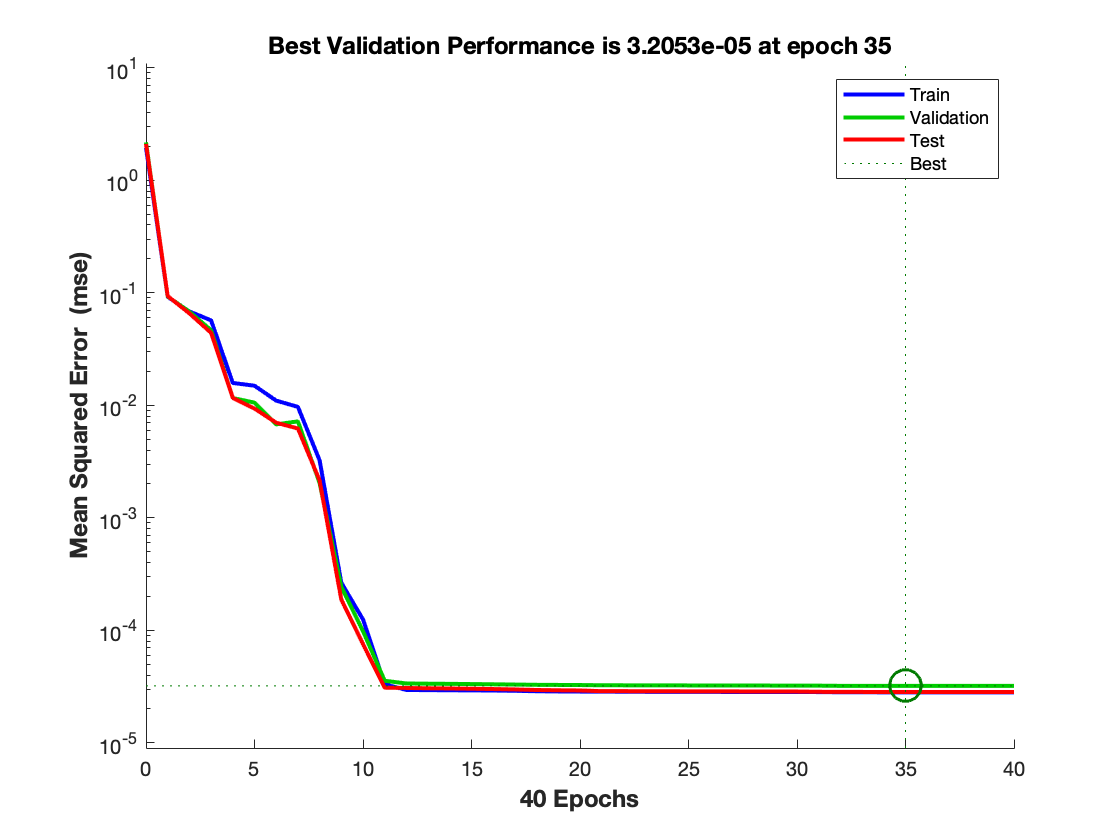
\includegraphics[width=20cm]{Epoch.png}
\end{figure}

\begin{figure}[h]
	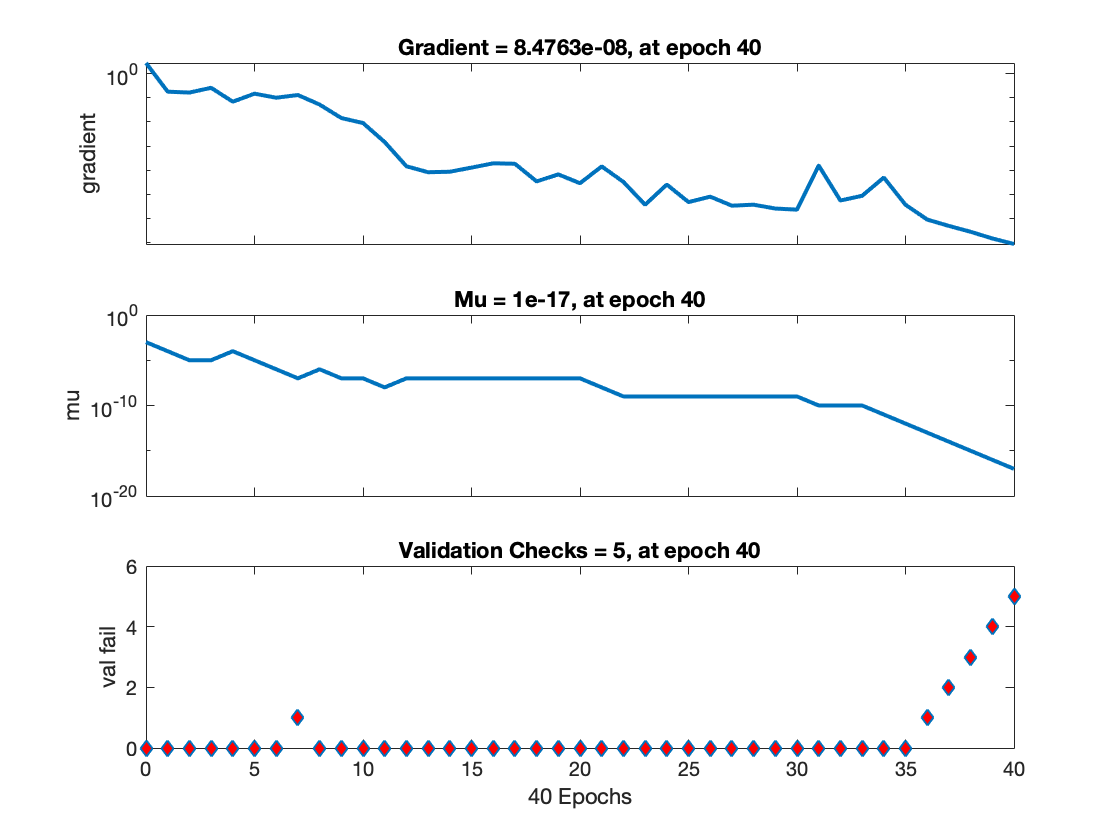
\includegraphics[width=20cm]{Training.png}
\end{figure}


\end{document}